% Created by tikzDevice version 0.10.1 on 2016-08-26 09:42:19
% !TEX encoding = UTF-8 Unicode
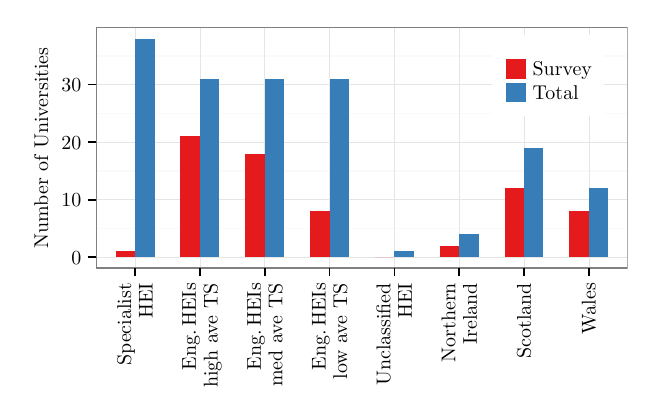
\begin{tikzpicture}[x=1pt,y=1pt]
\definecolor{fillColor}{RGB}{255,255,255}
\path[use as bounding box,fill=fillColor,fill opacity=0.00] (0,0) rectangle (216.81,130.09);
\begin{scope}
\path[clip] (  0.00,  0.00) rectangle (216.81,130.09);
\definecolor{drawColor}{RGB}{255,255,255}
\definecolor{fillColor}{RGB}{255,255,255}

\path[draw=drawColor,line width= 0.6pt,line join=round,line cap=round,fill=fillColor] (  0.00,  0.00) rectangle (216.81,130.09);
\end{scope}
\begin{scope}
\path[clip] ( 24.76, 43.19) rectangle (216.81,130.09);
\definecolor{fillColor}{RGB}{255,255,255}

\path[fill=fillColor] ( 24.76, 43.19) rectangle (216.81,130.09);
\definecolor{drawColor}{gray}{0.98}

\path[draw=drawColor,line width= 0.6pt,line join=round] ( 24.76, 57.53) --
	(216.81, 57.53);

\path[draw=drawColor,line width= 0.6pt,line join=round] ( 24.76, 78.32) --
	(216.81, 78.32);

\path[draw=drawColor,line width= 0.6pt,line join=round] ( 24.76, 99.11) --
	(216.81, 99.11);

\path[draw=drawColor,line width= 0.6pt,line join=round] ( 24.76,119.90) --
	(216.81,119.90);
\definecolor{drawColor}{gray}{0.90}

\path[draw=drawColor,line width= 0.2pt,line join=round] ( 24.76, 47.14) --
	(216.81, 47.14);

\path[draw=drawColor,line width= 0.2pt,line join=round] ( 24.76, 67.93) --
	(216.81, 67.93);

\path[draw=drawColor,line width= 0.2pt,line join=round] ( 24.76, 88.72) --
	(216.81, 88.72);

\path[draw=drawColor,line width= 0.2pt,line join=round] ( 24.76,109.51) --
	(216.81,109.51);

\path[draw=drawColor,line width= 0.2pt,line join=round] ( 38.81, 43.19) --
	( 38.81,130.09);

\path[draw=drawColor,line width= 0.2pt,line join=round] ( 62.23, 43.19) --
	( 62.23,130.09);

\path[draw=drawColor,line width= 0.2pt,line join=round] ( 85.65, 43.19) --
	( 85.65,130.09);

\path[draw=drawColor,line width= 0.2pt,line join=round] (109.07, 43.19) --
	(109.07,130.09);

\path[draw=drawColor,line width= 0.2pt,line join=round] (132.49, 43.19) --
	(132.49,130.09);

\path[draw=drawColor,line width= 0.2pt,line join=round] (155.92, 43.19) --
	(155.92,130.09);

\path[draw=drawColor,line width= 0.2pt,line join=round] (179.34, 43.19) --
	(179.34,130.09);

\path[draw=drawColor,line width= 0.2pt,line join=round] (202.76, 43.19) --
	(202.76,130.09);
\definecolor{fillColor}{RGB}{228,26,28}

\path[fill=fillColor] ( 31.78, 47.14) rectangle ( 38.81, 49.22);
\definecolor{fillColor}{RGB}{55,126,184}

\path[fill=fillColor] ( 38.81, 47.14) rectangle ( 45.84,126.14);
\definecolor{fillColor}{RGB}{228,26,28}

\path[fill=fillColor] ( 55.20, 47.14) rectangle ( 62.23, 90.80);
\definecolor{fillColor}{RGB}{55,126,184}

\path[fill=fillColor] ( 62.23, 47.14) rectangle ( 69.26,111.58);
\definecolor{fillColor}{RGB}{228,26,28}

\path[fill=fillColor] ( 78.63, 47.14) rectangle ( 85.65, 84.56);
\definecolor{fillColor}{RGB}{55,126,184}

\path[fill=fillColor] ( 85.65, 47.14) rectangle ( 92.68,111.58);
\definecolor{fillColor}{RGB}{228,26,28}

\path[fill=fillColor] (102.05, 47.14) rectangle (109.07, 63.77);
\definecolor{fillColor}{RGB}{55,126,184}

\path[fill=fillColor] (109.07, 47.14) rectangle (116.10,111.58);
\definecolor{fillColor}{RGB}{228,26,28}

\path[fill=fillColor] (125.47, 47.14) rectangle (132.49, 47.14);
\definecolor{fillColor}{RGB}{55,126,184}

\path[fill=fillColor] (132.49, 47.14) rectangle (139.52, 49.22);
\definecolor{fillColor}{RGB}{228,26,28}

\path[fill=fillColor] (148.89, 47.14) rectangle (155.92, 51.30);
\definecolor{fillColor}{RGB}{55,126,184}

\path[fill=fillColor] (155.92, 47.14) rectangle (162.94, 55.46);
\definecolor{fillColor}{RGB}{228,26,28}

\path[fill=fillColor] (172.31, 47.14) rectangle (179.34, 72.09);
\definecolor{fillColor}{RGB}{55,126,184}

\path[fill=fillColor] (179.34, 47.14) rectangle (186.36, 86.64);
\definecolor{fillColor}{RGB}{228,26,28}

\path[fill=fillColor] (195.73, 47.14) rectangle (202.76, 63.77);
\definecolor{fillColor}{RGB}{55,126,184}

\path[fill=fillColor] (202.76, 47.14) rectangle (209.78, 72.09);
\definecolor{drawColor}{gray}{0.50}

\path[draw=drawColor,line width= 0.6pt,line join=round,line cap=round] ( 24.76, 43.19) rectangle (216.81,130.09);
\end{scope}
\begin{scope}
\path[clip] (  0.00,  0.00) rectangle (216.81,130.09);
\definecolor{drawColor}{RGB}{0,0,0}

\node[text=drawColor,anchor=base east,inner sep=0pt, outer sep=0pt, scale=  0.72] at ( 19.36, 44.66) {0};

\node[text=drawColor,anchor=base east,inner sep=0pt, outer sep=0pt, scale=  0.72] at ( 19.36, 65.45) {10};

\node[text=drawColor,anchor=base east,inner sep=0pt, outer sep=0pt, scale=  0.72] at ( 19.36, 86.24) {20};

\node[text=drawColor,anchor=base east,inner sep=0pt, outer sep=0pt, scale=  0.72] at ( 19.36,107.03) {30};
\end{scope}
\begin{scope}
\path[clip] (  0.00,  0.00) rectangle (216.81,130.09);
\definecolor{drawColor}{RGB}{0,0,0}

\path[draw=drawColor,line width= 0.6pt,line join=round] ( 21.76, 47.14) --
	( 24.76, 47.14);

\path[draw=drawColor,line width= 0.6pt,line join=round] ( 21.76, 67.93) --
	( 24.76, 67.93);

\path[draw=drawColor,line width= 0.6pt,line join=round] ( 21.76, 88.72) --
	( 24.76, 88.72);

\path[draw=drawColor,line width= 0.6pt,line join=round] ( 21.76,109.51) --
	( 24.76,109.51);
\end{scope}
\begin{scope}
\path[clip] (  0.00,  0.00) rectangle (216.81,130.09);
\definecolor{drawColor}{RGB}{0,0,0}

\path[draw=drawColor,line width= 0.6pt,line join=round] ( 38.81, 40.19) --
	( 38.81, 43.19);

\path[draw=drawColor,line width= 0.6pt,line join=round] ( 62.23, 40.19) --
	( 62.23, 43.19);

\path[draw=drawColor,line width= 0.6pt,line join=round] ( 85.65, 40.19) --
	( 85.65, 43.19);

\path[draw=drawColor,line width= 0.6pt,line join=round] (109.07, 40.19) --
	(109.07, 43.19);

\path[draw=drawColor,line width= 0.6pt,line join=round] (132.49, 40.19) --
	(132.49, 43.19);

\path[draw=drawColor,line width= 0.6pt,line join=round] (155.92, 40.19) --
	(155.92, 43.19);

\path[draw=drawColor,line width= 0.6pt,line join=round] (179.34, 40.19) --
	(179.34, 43.19);

\path[draw=drawColor,line width= 0.6pt,line join=round] (202.76, 40.19) --
	(202.76, 43.19);
\end{scope}
\begin{scope}
\path[clip] (  0.00,  0.00) rectangle (216.81,130.09);
\definecolor{drawColor}{RGB}{0,0,0}

\node[text=drawColor,rotate= 90.00,anchor=base east,inner sep=0pt, outer sep=0pt, scale=  0.72] at ( 37.40, 37.79) {Specialist};

\node[text=drawColor,rotate= 90.00,anchor=base east,inner sep=0pt, outer sep=0pt, scale=  0.72] at ( 45.18, 37.79) {HEI};

\node[text=drawColor,rotate= 90.00,anchor=base east,inner sep=0pt, outer sep=0pt, scale=  0.72] at ( 60.82, 37.79) {Eng.\,HEIs};

\node[text=drawColor,rotate= 90.00,anchor=base east,inner sep=0pt, outer sep=0pt, scale=  0.72] at ( 68.60, 37.79) {high ave TS};

\node[text=drawColor,rotate= 90.00,anchor=base east,inner sep=0pt, outer sep=0pt, scale=  0.72] at ( 84.24, 37.79) {Eng.\,HEIs};

\node[text=drawColor,rotate= 90.00,anchor=base east,inner sep=0pt, outer sep=0pt, scale=  0.72] at ( 92.02, 37.79) {med ave TS};

\node[text=drawColor,rotate= 90.00,anchor=base east,inner sep=0pt, outer sep=0pt, scale=  0.72] at (107.66, 37.79) {Eng.\,HEIs};

\node[text=drawColor,rotate= 90.00,anchor=base east,inner sep=0pt, outer sep=0pt, scale=  0.72] at (115.44, 37.79) {low ave TS};

\node[text=drawColor,rotate= 90.00,anchor=base east,inner sep=0pt, outer sep=0pt, scale=  0.72] at (131.09, 37.79) {Unclassified};

\node[text=drawColor,rotate= 90.00,anchor=base east,inner sep=0pt, outer sep=0pt, scale=  0.72] at (138.86, 37.79) {HEI};

\node[text=drawColor,rotate= 90.00,anchor=base east,inner sep=0pt, outer sep=0pt, scale=  0.72] at (154.51, 37.79) {Northern};

\node[text=drawColor,rotate= 90.00,anchor=base east,inner sep=0pt, outer sep=0pt, scale=  0.72] at (162.28, 37.79) {Ireland};

\node[text=drawColor,rotate= 90.00,anchor=base east,inner sep=0pt, outer sep=0pt, scale=  0.72] at (181.82, 37.79) {Scotland};

\node[text=drawColor,rotate= 90.00,anchor=base east,inner sep=0pt, outer sep=0pt, scale=  0.72] at (205.24, 37.79) {Wales};
\end{scope}
\begin{scope}
\path[clip] (  0.00,  0.00) rectangle (216.81,130.09);
\definecolor{drawColor}{RGB}{0,0,0}

\node[text=drawColor,rotate= 90.00,anchor=base,inner sep=0pt, outer sep=0pt, scale=  0.72] at (  7.36, 86.64) {Number of Universities};
\end{scope}
\begin{scope}
\path[clip] (  0.00,  0.00) rectangle (216.81,130.09);
\definecolor{fillColor}{RGB}{255,255,255}

\path[fill=fillColor] (167.86, 98.10) rectangle (208.15,127.32);
\end{scope}
\begin{scope}
\path[clip] (  0.00,  0.00) rectangle (216.81,130.09);
\definecolor{fillColor}{RGB}{228,26,28}

\path[fill=fillColor] (172.83,111.61) rectangle (179.95,118.72);
\end{scope}
\begin{scope}
\path[clip] (  0.00,  0.00) rectangle (216.81,130.09);
\definecolor{fillColor}{RGB}{55,126,184}

\path[fill=fillColor] (172.83,103.08) rectangle (179.95,110.19);
\end{scope}
\begin{scope}
\path[clip] (  0.00,  0.00) rectangle (216.81,130.09);
\definecolor{drawColor}{RGB}{0,0,0}

\node[text=drawColor,anchor=base west,inner sep=0pt, outer sep=0pt, scale=  0.72] at (182.47,112.69) {Survey};
\end{scope}
\begin{scope}
\path[clip] (  0.00,  0.00) rectangle (216.81,130.09);
\definecolor{drawColor}{RGB}{0,0,0}

\node[text=drawColor,anchor=base west,inner sep=0pt, outer sep=0pt, scale=  0.72] at (182.47,104.15) {Total};
\end{scope}
\end{tikzpicture}
